%!TEX root = ../../main.tex

\chapter{Entwurf} % oder Entwicklung
In diesem Kapitel wird der Entwurf und die Architektur des Programms beschrieben. Zuerst wird beschrieben, welche Anforderungen es an das Programm gibt. Danach werden die verwendeten Architekturpatterns erläutert. Darauf folgt ein Kapitel zur Architektur des Backends in dem beschrieben wird, wie die Endpunkte der API gestaltet sind, welche Technologien verwendet werden und wie der innere Aufbau der API gestaltet ist. Anschließend werden die wichtigsten Prozesseabläufe dargestellt und schließlich, wie das Projekt auf einem Server aufgesetzt wird.

\section{Anforderungen}
Das Programm soll eine Webanwendung sein auf der Nutzer mit einer benutzerfreundlichen Oberfläche verschiedene Eröffnungen betrachten und trainieren können. Es soll dabei als zentraler Ort dienen um Eröffnungen nachzuschauen und sein Gedächtnis aufzufrischen. Die Anwendung unterstützt Lernende, indem sie personalisiert Vorschläge gibt, welche Eröffnungen erneut geübt werden sollen. Es gelten für sie folgende funtkionale Anforderungen:

\begin{itemize}
    \item Login: Ein Nutzer kann sich bei der Anwendung anmelden.
    \item Registrieren: Ein Nutzer kann sich einen Account anlegen.
    \item Spielumfang: Die Anwendung bietet zu Beginn jeweils eine Eröffnung für die weißen und für die schwarzen Figuren an.
    \item Lernmodus: Ein Nutzer kann eine Eröffnung auswählen und anschließend verschiedene Zugfolgen und Varianten der Eröffnung betrachten.
    \item Übungsmodus: Ein Nutzer kann eine Eröffnung auswählen und muss dann die Figuren einer Farbe nach der Zugfolge der Eröffnung bewegen. Der Computer spielt dabei die Züge des Gegners.
    \item Übungsmodus Hinweise: Während dem Üben hat ein Nutzer die Möglichkeit sich Hinweise geben zu lassen.
    \item Übungsmodus Erweiterung: Ein Nutzer hat die Möglichkeit nach einer Eröffnung mit oder ohne Dekomposition das Spiel zu Ende zu spielen gegen einen Computergegner.
    \item Vorschläge: Ein Nutzer bekommt Vorschläge welche Eröffnung trainiert werden soll.
    \item Statistik: Ein Nutzer kann sich Statistiken zu den Eröffnungen anschauen. Dazu zählt die Anzahl an richtigen und falschen Übungsdurchläufen. Diese Statistik wird auch zur Erstellung der Vorschläge verwendet.
\end{itemize}

\section{Patterns}
In diesem Kapitel werden architekturübergreifende Patterns vorgestellt, die unabhängig vom gewählten Architekturstil eingesetzt werden können. Sie tragen dazu bei, den Code besser strukturiert, wartbar und erweiterbar zu gestalten. Dazu gehören das Repository Pattern und Dependency Injection. Beide Patterns werden im Folgenden anhand ihrer Funktion und ihres Einsatzes im Projekt erläutert.

\subsection{Repository Pattern}
Um die Datenspeicherung von dem Rest des Backends zu trennen wird das Repository Pattern angewendet. Bei diesem Pattern wird eine Repository-Klasse erstellt, welche die Abfragelogik enthält. Nach außen werden nur abstrakte domänenspezifische Funktionen exponiert, wie zum Beispiel \lstinline{GetUser(id: int): User} oder \lstinline{CreateUser(name: string, password: string)}. Die Implementierung dieser Klasse sorgt dann dafür, dass die entsprechenden Daten gefunden, aktualisiert oder hinzugefügt werden. Diese Abfragen können zum Beispiel komplexe SQL-Abfragen sein oder auch das Lesen einer Datei. In diesem Projekt wird jede Repository durch ein Interface definiert. Das ermöglicht es die jeweiligen Implementierungen mittels Dependency Injection zu ersetzen. \cite{evans_domain-driven_2004}
\missingfigure{Beispieldiagramm}

\subsection{Dependency Injection}
\todo{TODO}

\section{Architektur}
Die Architektur ist in mehrere verschiedene Bestandteile aufgeteilt. Die zentrale Aufteilung besteht zwischen Backend und Frontend. In dieser Arbeit wird nur das Backend betrachtet. In \autoref{fig:components} ist ein Überblick über die Architektur zu sehen. Das Frontend greift auf eine \ac{REST}-API zu.
Die API ist wiederum aufgeteilt in die vier Bestandteile Eröffnungen, Nutzerdaten, Statistiken und die Schachengine.
Die Bestandteile werden in den folgenden Unterkapiteln näher erklärt.
% Der Bestandteil Eröffnungen ist für alles zuständig, wofür die Daten für Eröffnungen benötigt werden. Dazu gehört also das Lernen und Üben von Eröffnungen. Der Bestandteil Nutzerdaten ist notwendig um das Registrieren und den Login zu ermöglichen und die Statistiken sind nützlich um den Fortschritt der Spieler zu verfolgen und ermöglichen eine personalisierte Anpassung der Lernerfahrung. Die Schachengine ist notwendig für das Spielen gegen den Computer.

\begin{figure}[h]
    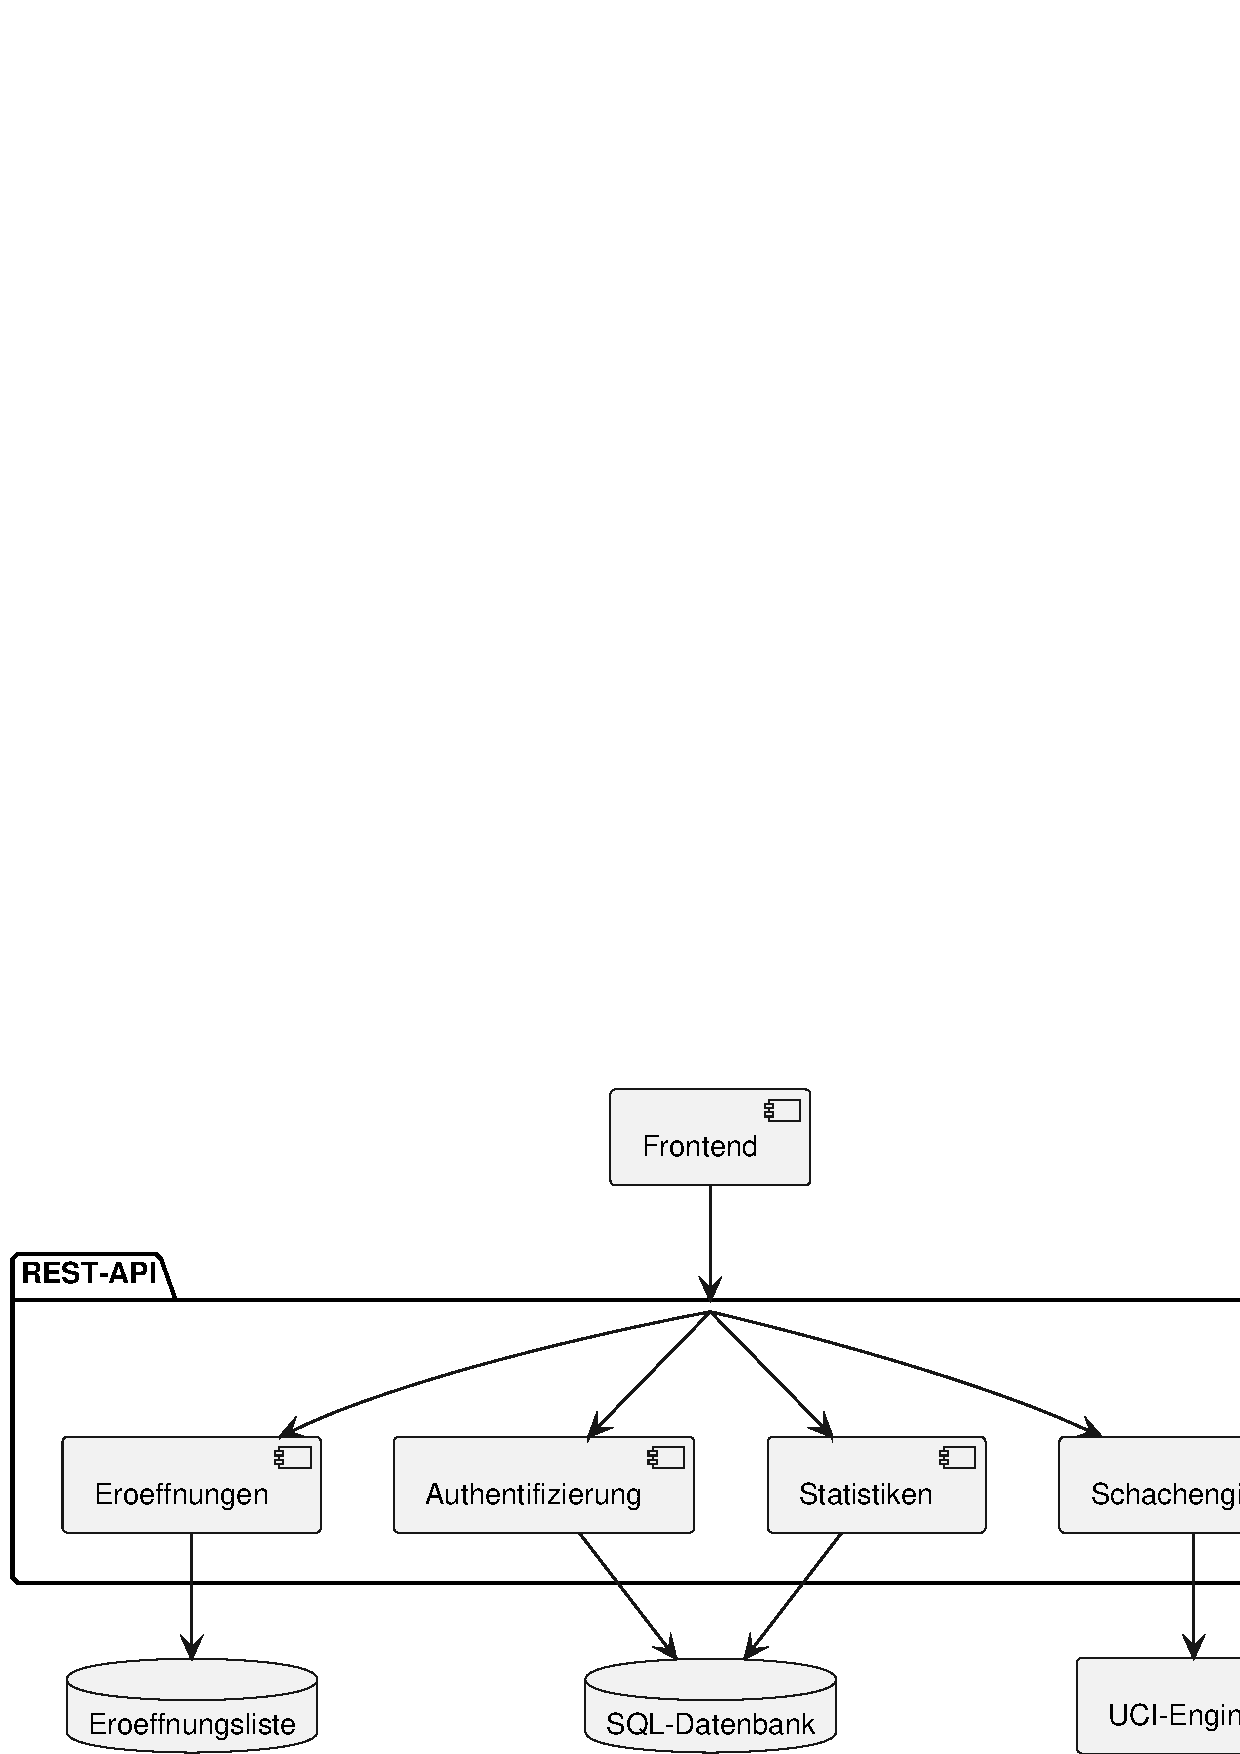
\includegraphics[width=\linewidth]{images/diagrams/components.png}
    \caption{Komponentendiagramm}
    \label{fig:components}
\end{figure}

\subsection{REST-API}
Die API wird in C\# realisiert. Mit dem ASP.NET Core Framework wird eine controllerbasierte Web-API erstellt. Das bedeutet, dass die Controller und die Daten voneinander getrennt werden. Die Architektur ist ähnlich, wie eine Model View Controller Architektur, mit dem Unterschied, dass es keine View gibt. Die View wird separat im Frontend entwickelt. Die Controller und die Models sind im Backend vorhanden. Die Controller offenbaren die API-Endpunkte nach außen und die Models modellieren die Daten. Für die vier unterschiedlichen Bereiche des Backends existiert jeweils ein dazugehöriger Controller. Jeder Controller repräsentiert dabei einen Wurzelendpunkt in der REST-API. Damit gibt es die vier Wurzelendpunkte \lstinline{/engine}, \lstinline{/openings}, \lstinline{/users} und \lstinline{/stats}. Ein Controller-Endpunkt gibt immer ein \lstinline{IActionResult} zurück. Wenn in der Implementierung ein anderer Datentyp zurückgegeben wird, kümmert sich das Framework darum, dass er umgewandelt wird. Das resultiert in einem \lstinline{OkObjektResult} mit dem Statuscode 200 und dem zurückgegebenen Objekt als Wert. Dieses Objekt wird vor der Antwort in JSON umgewandelt. Um Verständlichkeit der nachfolgenden Klassendiagramme zu erhöhen wird nur der Datentyp dieses Objekts dargestellt. In manchen Fällen ist es auch möglich, dass statt des Datentyps eine Antwort mit Fehlercode und anderen Daten übergeben wird. Das wird an den entsprechenden Stellen beschrieben und ist auch in der OpenAPI Dokumentation zu sehen.
% TODO im Code umsetzen

\subsection{Eröffnungen}
\label{cp:openings}
Der Bestandteil Eröffnungen ist für alles zuständig, wofür die Daten der Eröffnungen benötigt werden. Dazu gehört also das Lernen und Üben von Eröffnungen. \autoref{fig:cd_opening} zeigt die dazugehörigen Klassen.

\subsubsection{OpeningController}
Der OpeningController definiert alle Endpunkte unter der URI \lstinline{/openings}.
Jede public Funktion der Klasse ist in diesem Fall für einen Endpunkt zuständig. Die Zuteilung ist folgendermaßen gestaltet:

\begin{itemize}
  \item \lstinline|GET /openings| $\rightarrow$ GetOpenings
  \item \lstinline|GET /openings/{id}/variant| $\rightarrow$ GetVariants
  \item \lstinline|GET /openings/{id}/variant/next-moves| $\rightarrow$ GetMoveVariants
  \item \lstinline|GET /openings/{id}/next-move| $\rightarrow$ GetNextMove
\end{itemize}

Der Endpunkt \lstinline{GET /openings} liefert eine Liste mit allen Wurzeleröffnungen in Form von OpeningOverview-Objekten, die jeweils den Namen und die ID einer Eröffnung enthalten.
Eine Eröffnung wird dann als Wurzeleröffnung kategorisiert, wenn der Name keinen Doppelpunkt enthält. %todo braucht das weitere Erklärung?

Der Endpunkt \lstinline|GET /openings/{id}/variant| ist dazu da alle Eröffnungen einer Eröffnungsfamilie zu bekommen. Eine Eröffnung gilt als zugehörig zu dieser Familie, wenn sie mit dem Namen beginnt, den Eröffnung mit der gegebenen ID besitzt. Zum Beispiel besitzt die Eröffnung mit der ID D20 den Namen \enquote{Queen's Gambit Accepted}. Das bedeutet alle Eröffnungen, die mit diesem Namen beginnen gehören zu dieser Familie.

Der Endpunkt \lstinline|GET /openings/{id}/next-move| gibt ein OpeningMove-Objekt zurück, dass den Namen der Eröffnung und den nächsten Zug enthält. Bei diesem Endpunkt kann zusätzlich das Query-Parameter played übergeben werden mit den bisher gespielten Zügen im \ac{UCI}-Format. Wenn alle Züge gespielt wurden, wird ein leerer String als Zug übergeben.

Der Endpunkt \lstinline|GET /openings/{id}/variant/next-moves| dient dazu alle möglichen nächsten Züge in einer Eröffnungsfamilie herauszufinden. Er gibt alle OpeningMove-Objekte der gegebenen Eröffnungsfamilie zurück. Auch hier kann man das Query-Parameter played mitgeben. Die Liste enthält dann nur noch die Eröffnungen, die auch mit diesen Zügen beginnen.Beispielsweise werden bei der Anfrage \lstinline|GET /openings/D20/variant|

% Die Zuordnung zu einer Eröffnungsfamilie findet statt, wie in \autoref{cp:opening list} beschrieben.

\subsubsection{OpeningRepository}
Opening ist die Model Klasse. Sei enthält alle benötigten Daten zu einer Eröffnung. Die API gibt bei einer Anfrage entweder Instanzen der Klassen OpeningOverview oder OpeningMove zurück, die einen Teil der Informationen von Opening besitzen. Dadurch wird Bandbreite gespart und der Client bekommt nur die Daten, die er auch benötigt. Der Datenspeicher ist eine TSV-Datei, die von dem Lichess Datensatz abgeleitet wurde. %todo genauer beschreiben wie er abgeleitet wurde?
Er wird über das Repository Pattern abgefragt. IOpeningRepository enthält also alle Funtionen, um die Daten abzufragen und zu strukturieren, wie sie der OpeningController benötigt. Die OpeningRepository verwendet wiederum den IOpeningReader, welcher das Lesen der TSV-Datei abstrahiert. Auf diese Weise kann die TSV-Datei ohne viel Aufwand durch eine CSV- oder JSON-Datei ausgetauscht werden. Dafür muss lediglich eine entsprechende Implementierung für den IOpeningReader erstellt werden.

\begin{figure}[h]
  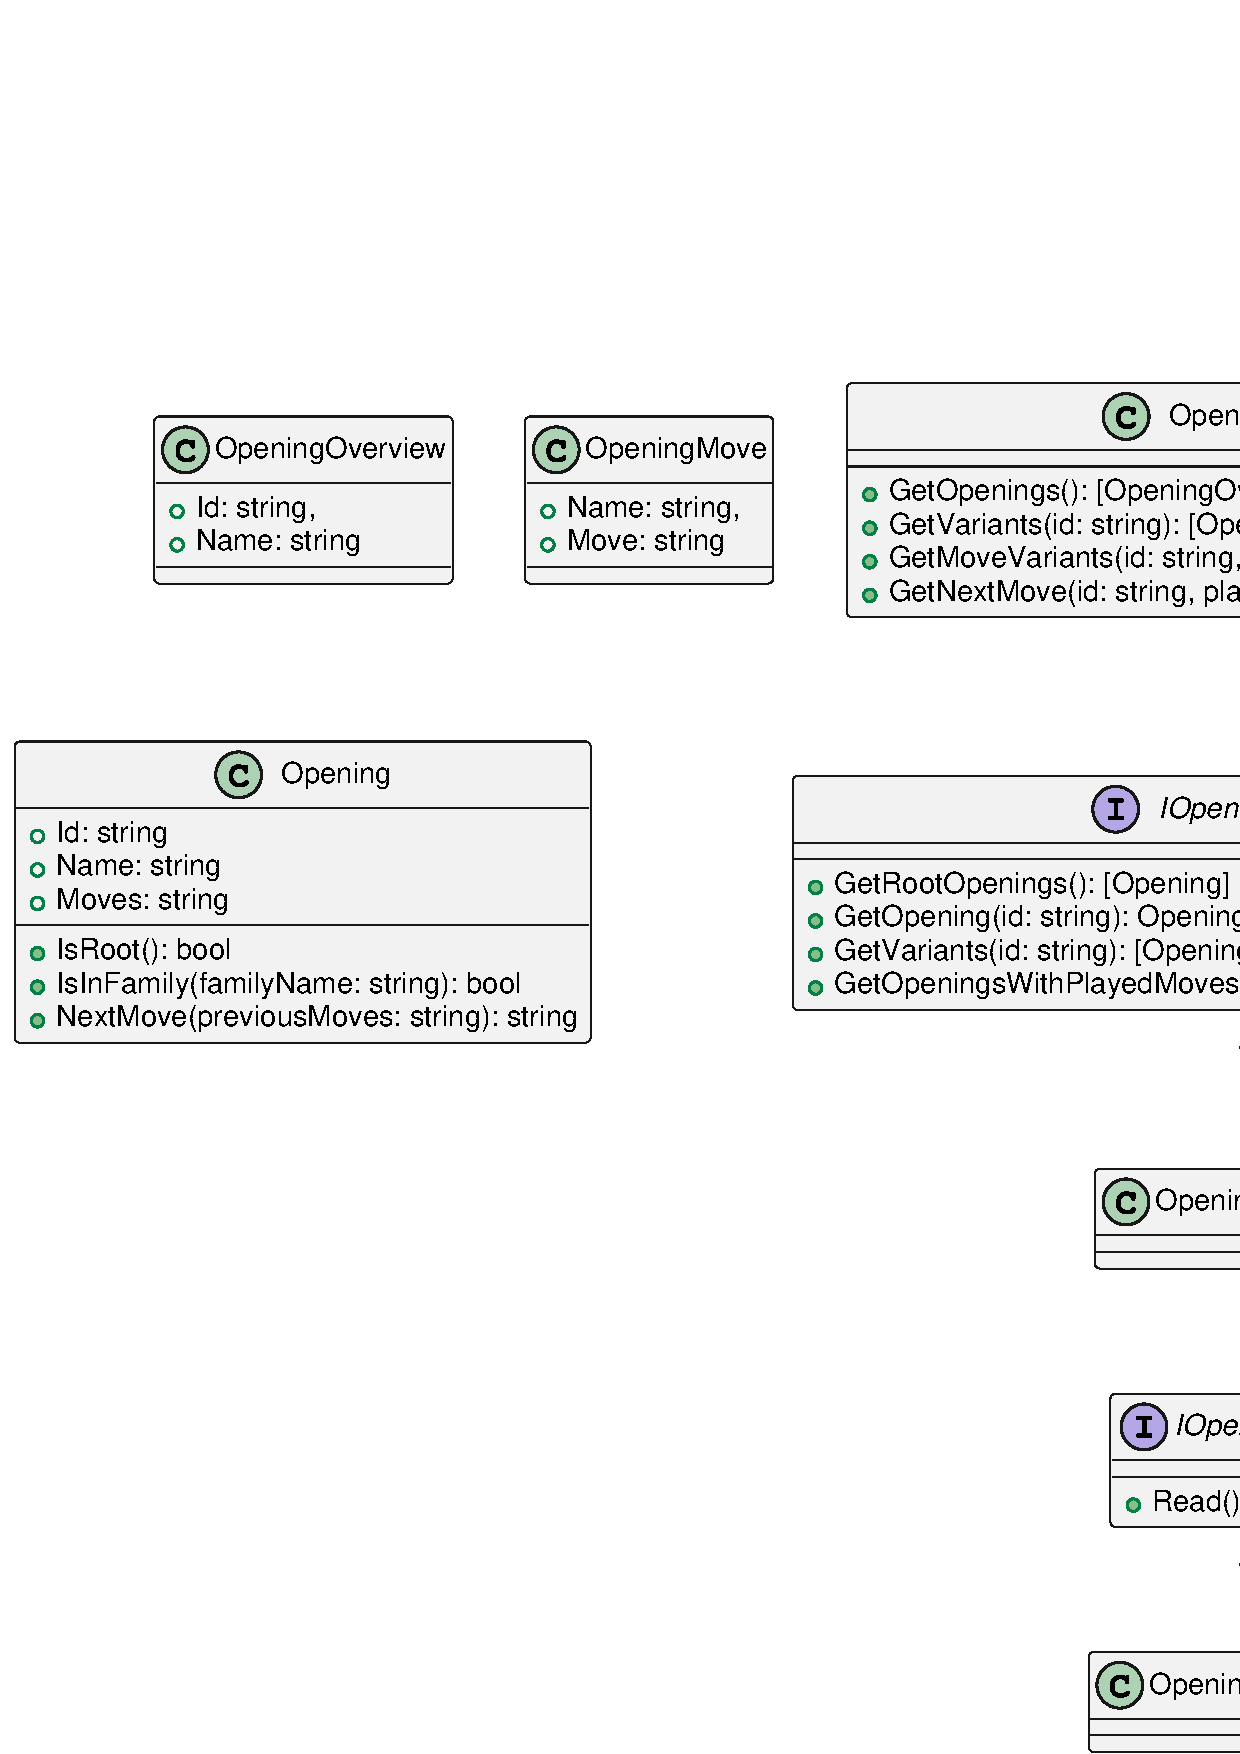
\includegraphics[width=\linewidth]{images/diagrams/opening.png}
  \caption{Klassendiagramm Eröffnungen}
  \label{fig:cd_opening}
\end{figure}

\subsection{SQL-Datenbank}
Die dynamischen Daten werden in einer relationalen SQL-Datenbank gespeichert. Dazu zählen die Logindaten der Nutzer und die Nutzerstatistiken zu den Eröffnungen. Dafür existieren die zwei Tabellen User und TrainingResult, welche nachfolgend in Relationenschreibweise notiert sind, wobei der Primärschlüssel fett gedruckt ist und der Fremdschlüssel kursiv:

\begin{itemize}
  \item User(\textbf{Id}, Name, PasswordHash)
  \item TrainingResult(\textbf{Id}, \textit{UserId}, OpeningId, Errors, Hints, DateTime)
\end{itemize}

Die Usertabelle existiert um das Einloggen und Registrieren zu ermöglichen. Mit einem Benutzernamen und einem Passwort kann sich ein Nutzer anmelden. Der Name besitzt aus diesem Grund einen Unique Constriant. Das Passwort wird in gehashter Form gespeichert. Für die Statistiken werden die Ergebnisse der Trainings gespeichert. Es wird gespeichert, wer das Training ausgeführt hat, für welche Eröffnung das Training ist, wie viele Fehler gemacht wurden, wie viele Hinweise benötigt wurden und zu welchem Zeitpunkt das Training ausgeführt wurde. OpeningId ist in diesem Fall kein Fremdschlüssel, da die Eröffnungen nicht in der relationalen Datenbank abgespeichert sind, sondern in einer separaten TSV-Datei. Mithilfe dieser Daten können durch SQL-Abfragen beliebige Statistiken erstellt werden.

Für den Datenbankzugriff wird ein \ac{ORM} verwendet. Microsoft bietet in C\# dafür das Entity Framework Core an. Der Vorteil eines \ac{ORM}s ist, dass es den Zugriff auf die Datenbank abstrahiert. Zwischen verschiedenen SQL-Datenbanken gibt es einige Unterschiede, auf die geachtet werden muss, beim Schreiben von reinem SQL. Ein \ac{ORM} abstrahiert diese Unterschiede, indem der Zugriff und die Tabellenstruktur in der Sprache des ORM-Frameworks beschrieben wird, in diesem Fall C\#. Ein weiterer Vorteil ist, dass \ac{ORM}s vor einigen Fehlern, wie zum Beispiel Query-Injection schützen. Das Entity Framework Core besitzt zudem ein robustes System für Datenbankmigrationen. So ist es möglich Tabellenstrukturen auch im Nachhinein zu ändern und die Datenbanken mit geringem Risiko zu migrieren. Mit dem Entity Framework Core kann man zwischen vielen SQL-Datenbanken wählen. Für dieses Projekt wird PostgreSQL verwendet, da sie weit verbreitet ist und bekannt für ihre Stabilität.

\subsection{Authentifizierung}
Wie bereits in \autoref{cp:auth} beschrieben, wird auch in diesem Projekt eine Authentifizierung der Nutzer benötigt, zum einen, um nutzerbezogene Statistiken zu sammeln und eine personalisierte Erfahrung zu bieten, zum anderen, um den Zugriff auf die Schachengine zu begrenzen. \autoref{fig:cd_auth} beschreibt die Klassen, die bei der Authentifizierung verwendet werden. Der \lstinline{UserController} implementiert die folgende Endpunkte:

\begin{itemize}
    \item \lstinline{POST /users} $\rightarrow$ CreateUser
    \item \lstinline{POST /users/login} $\rightarrow$ Login
\end{itemize}

Über den ersten Endpunkt geschieht die Registrierung. Das Frontend schickt mit einer POST Anfrage den Nutzername, der angelegt werden soll und das Passwort. Der Nutzername besitzt in der Datenbank einen Unique Index, damit jeder Name nur einmal existiert. Dadurch ist es später möglich, sich mit Name und Passwort zu authentifizieren.
Wenn der angegebene Nutzername bereits existiert, wird eine Fehlermeldung mit dem Code 409 (Conflict) geschickt, da es sich um einen semantischen Fehler handelt und die Anfrage im Konflikt mit dem Zustand des Servers steht. %todo richtigen Fehlercode im Code verwenden
Wenn der Nutzer noch nicht existiert, wird er mithilfe der Klasse UserRepository angelegt.
% Sie verwendet den Passworthasher von ASP.NET Core, welcher eine sichere Hashfunktion mit Salt verwendet, um die Passwörter sicher zu speichern.
Zur sicheren Speicherung der Passwörter wird der Passwort-Hasher von ASP.NET Core verwendet, der eine sichere Hashfunktion mit einem zufällig generierten Salt verwendet.

Die erste Authentifizierung wird über den Controller-Endpunkt \lstinline{POST /users/login} durchgeführt. Dafür muss der eindeutige Nutzername und das Passwort angegeben werden. Der UserController kann mithilfe des UserRepositorys überprüfen, ob der Nutzer existiert und ob das angegebene Passwort richtig ist. Dafür wird wieder die selbe Hashfunktion genutzt. Falls eine der Überprüfungen fehlschlägt, wird eine Fehlermeldung mit dem Code 401 (Unauthorized) zurückgeschickt. Andernfalls wird über die Funktion GenerateJWT ein \ac{JWT} erstellt. Dieses Token enthält die User ID und den Ablaufzeitpunkt, welcher initial zwei Stunden in der Zukunft liegt. Der Ablaufzeitpunkt ist wichtig, damit das Token nicht auf unbestimmte Zeit gültig bleibt und somit ein Sicherheitsrisiko birgt. Weitere Informationen und komplexere Nutzerrollen sind in dieser Anwendung nicht notwendig. Mithilfe von diesem Token kann der Nutzer die weiteren Endpunkte verwenden, die auch eine Authentifizierung benötigen. Das ist bei allen der Fall, außer bei den Endpunkten des UserControllers, um die Angriffsfläche zu minimieren.

\begin{figure}
    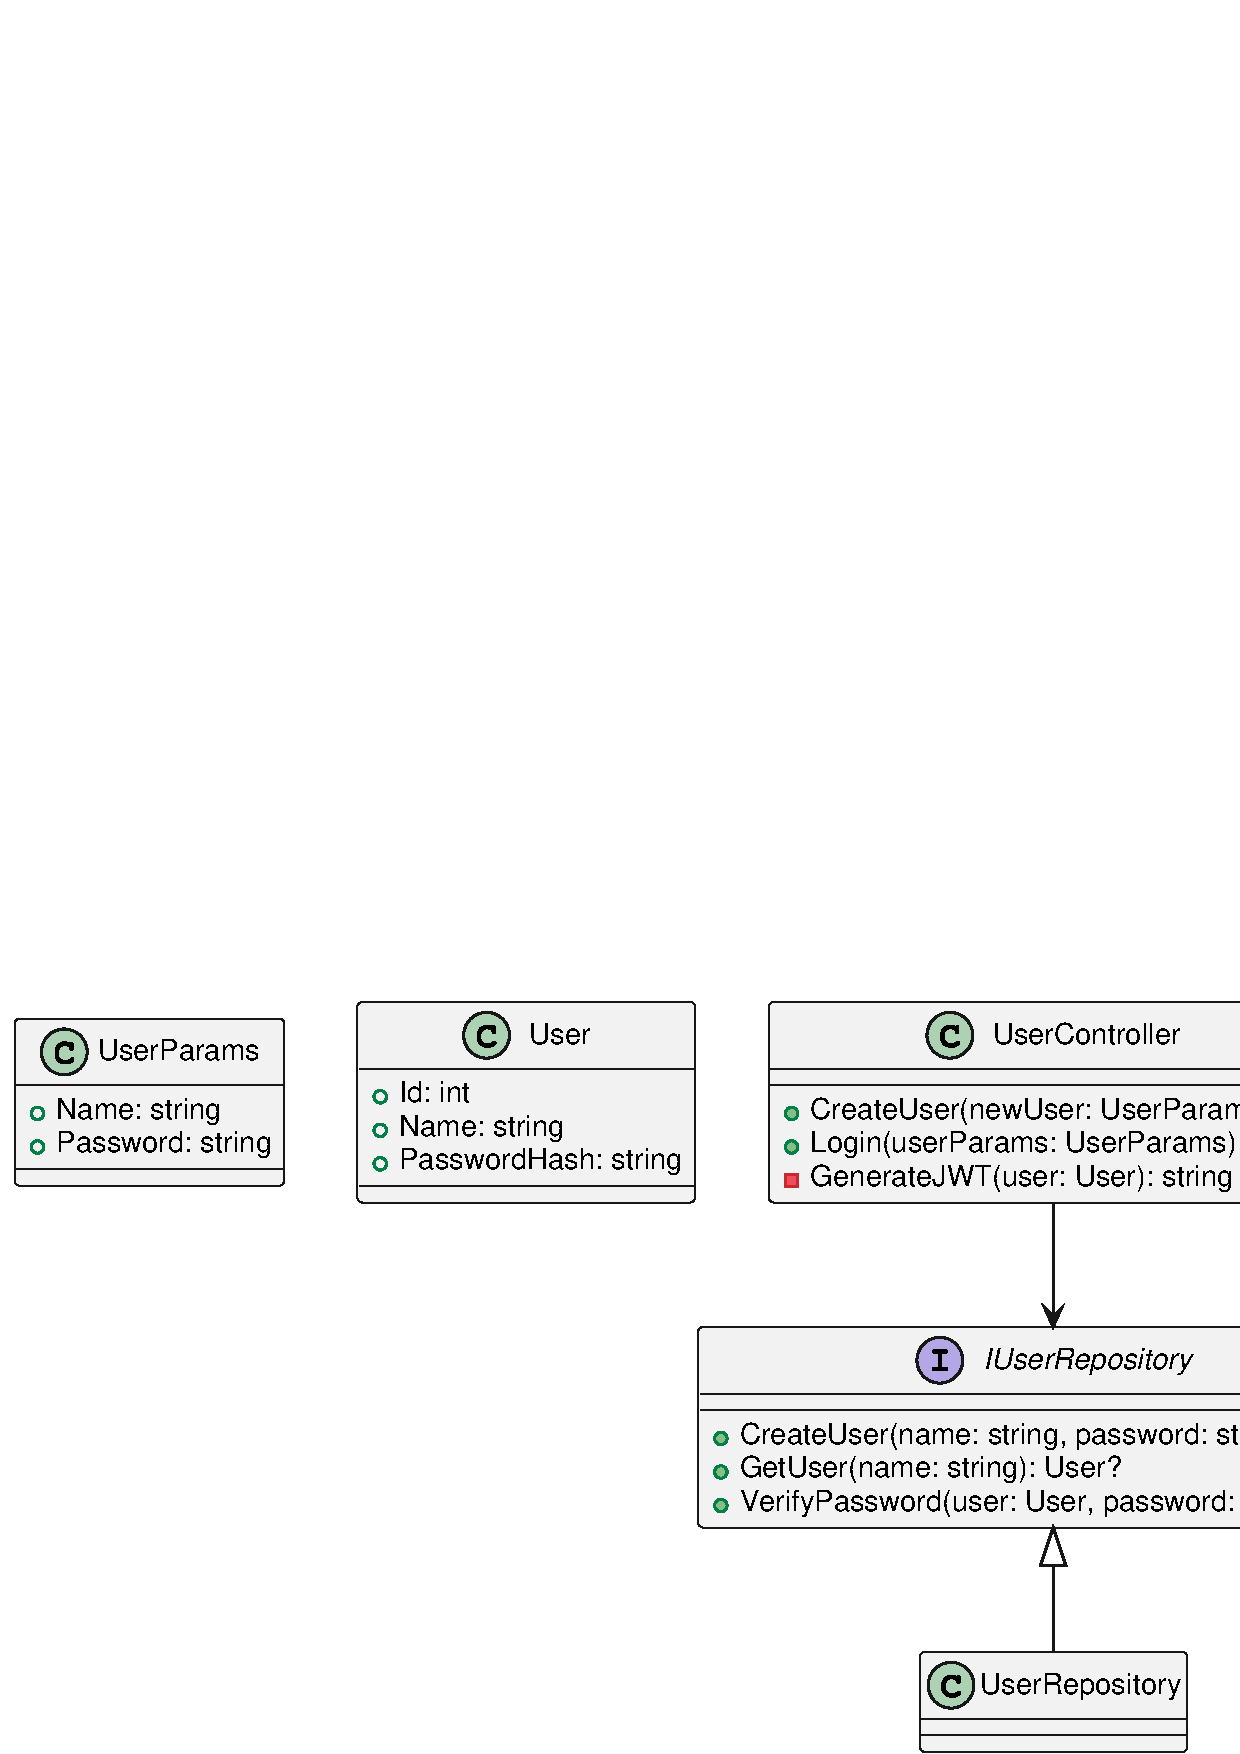
\includegraphics[width=\linewidth]{images/diagrams/auth.png}
    \caption{Klassendiagramm Authentifizierung}
    \label{fig:cd_auth}
\end{figure}

\subsection{Statistiken}
\todo{TODO}

\subsection{Schachengine}
\todo{TODO}

\section{Laufzeitsicht}

In diesem Kapitel wird der Ablauf von den komplexeren Funktionen der Anwendung beschrieben. Dabei wird erklärt, welche Anfragen das Frontend schickt und wie die REST-Endpunkte dabei verwendet werden.

\subsection{Lernmodus}
Für den Lernmodus werden die Funktionen unter dem Endpunkt \lstinline{/openings} aus \autoref{cp:openings} verwendet.
Der Ablauf des Lernmodus ist in \autoref{fig:sd_opening_training} dargestellt. Er kann in den folgenden drei Schritten zusammengefasst werden.

\begin{enumerate}
     \item Als erstes wählt der Nutzer den Lernmodus aus. Das Frontend schickt dann eine GET Anfrage an den Endpunkt \lstinline{/openings}. Dieser liefert eine Liste von OpeningOverviews, was Objekte sind, die die Namen und IDs der Wurzeleröffnungen darstellen. Diese Namen werden dem Nutzer zur Auswahl gezeigt.
     \item Angenommen der Nutzer wählt die Eröffnung mit der ID D20 aus. Dann schickt das Frontend eine GET Anfragen an den Endpunkt \lstinline|/openings/D20/variants/next-moves|. Daraufhin liefert die API ein OpeningMove-Objekt für jede Eröffnung, die mit dem selben Namen anfangen, wie die Eröffnung mit der ID D20. Die OpeningMove-Objekte enthalten den Namen und den ersten Zug der jeweiligen Eröffnung. Diese werden dem Nutzer angezeigt.
     \item Der Nutzer kann anschließend auswählen, welchen Zug er ausführen möchte, zum Beispiel 1. d4. Die darauffolgenden Züge können wiederum mit der folgenden GET Anfrage herausgefunden werden: \lstinline|/openings/D20/variants/next-moves?played=d2d4|. Hier werden die bereits ausgeführten Züge im Query-Parameter \lstinline{played} mit \ac{UCI}-Format übergeben. Die API liefert dann nur noch die Eröffnungen, die auch mit den selben Zügen beginnen. Dieser Schritt wird so oft wiederholt, bis keine weiteren Züge mehr vorhanden sind, also die Liste mit OpeningMoves leer ist.
\end{enumerate}

\begin{figure}
    \includegraphics[width=\linewidth]{images/diagrams/sd_opening_training}
    \caption{Ablauf Übungsmodus}
    \label{fig:sd_opening_training}
\end{figure}

\subsection{Übungsmodus}
Der Übungsmodus hat einen ähnlichen Ablauf, wie der Lernmodus und verwendet ähnliche Endpunkte. Statt dem Endpnkt \lstinline|/openings/{id}/variants/next-moves| wird hier der Endpunkt \lstinline|/openings/{id}/next-move| verwendet, da nicht die unterschiedlichen Varianten betrachtet werden müssen. Der letztere Endpunkt liefert nur ein OpeningMove-Objekt statt einer Liste. Auch bei diesem Endpunkt kann das Query-Parameter played übergeben werden mit den gespielten Zügen im \ac{UCI}-Format. Wenn es die passenden Züge waren, wird ein OpeningMove-Objekt mit dem nächsten Zug zurückgegeben oder ein 

\begin{enumerate}
    \item Als erstes wählt der Nutzer den Übungsmodus aus und das Frontend holt sich wieder über \lstinline{GET /openings} die Liste der Eröffnungen in Form von OpeningOverview-Objekten und zeigt diese mit Namen an.
    \item Der Nutzer wählt diesmal aus, welche Eröffnung er üben will und ob er die schwarzen Figuren oder die weißen spielen will. Bei Auswahl der weißen Figuren geht es mit Schritt 3 weiter, bei Auswahl der schwarzen mit Schritt 4.
    \item Für den nächsten Zug wird der Nutzer aufgefordert, ihn auszuführen. Das Frontend fragt daraufhin mit dem Endpunkt \lstinline|GET /openings/{id}/next-move| ab, was der richtige nächste Zug für diese Eröffnung ist. Die Antwort der API ist hier auch ein OpeningMove-Objekt mit dem Namen der Eröffnung und dem nächsten Zug als Inhalt. Wenn die Züge nicht übereinstimmen, wird der Nutzer aufgefordert es erneut zu versuchen. An dieser Stelle kann auch die Hinweisfunktion implementiert werden. Wenn der Nutzer nach einem Hinweis fragt, kann das Frontend über den selben Endpunkt den richtigen Zug abfragen und einen Hinweis geben, wie zum Beispiel, welche Figur bewegt werden muss. Dafür ist kein zusätzlicher Endpunkt in der API notwendig.


    \item Wenn der Spieler den richtigen Zug gefunden hat, holt das Frontend den nächsten Zug
    \item Wenn der Spieler den richtigen Zug gefunden hat, wird er aufgefordert, den nächsten Zug auszuführen. Der nächste Zug kann, ähnlich wie im Lernmodus, von der API geholt werden, indem das Query-Parameter played mit den gespielten Zügen im \ac{UCI}-Format mit übergeben wird, zum Beispiel: \lstinline{GET /openings/D20/next-move?played=d2d4%20d}
\end{enumerate}

% Diesmal wird im der erste Zug nicht gezeigt, sondern er muss ihn selber ausführen. Das Frontend frägt daraufhin mit dem Endpunkt \lstinline|GET /openings/{id}/next-move| ab, was der richtige Zug für diese Eröffnung ist. Wenn die Züge nicht übereinstimmen, wird der Nutzer aufgefordert es erneut zu versuchen. An dieser Stelle kann auch die Hinweisfunktion implementiert werden. Wenn der Nutzer nach einem Hinweis fragt, kann das Frontend über den selben Endpunkt den richtigen Zug abfragen und einen Hinweis geben, wie zum Beispiel, welche Figur bewegt werden muss. Dafür ist kein zusätzlicher Endpunkt in der API notwendig.

Als erstes wählt der Nutzer wieder die Eröffnung, über die er abgefragt werden will.

\begin{figure}
    \begin{center}
        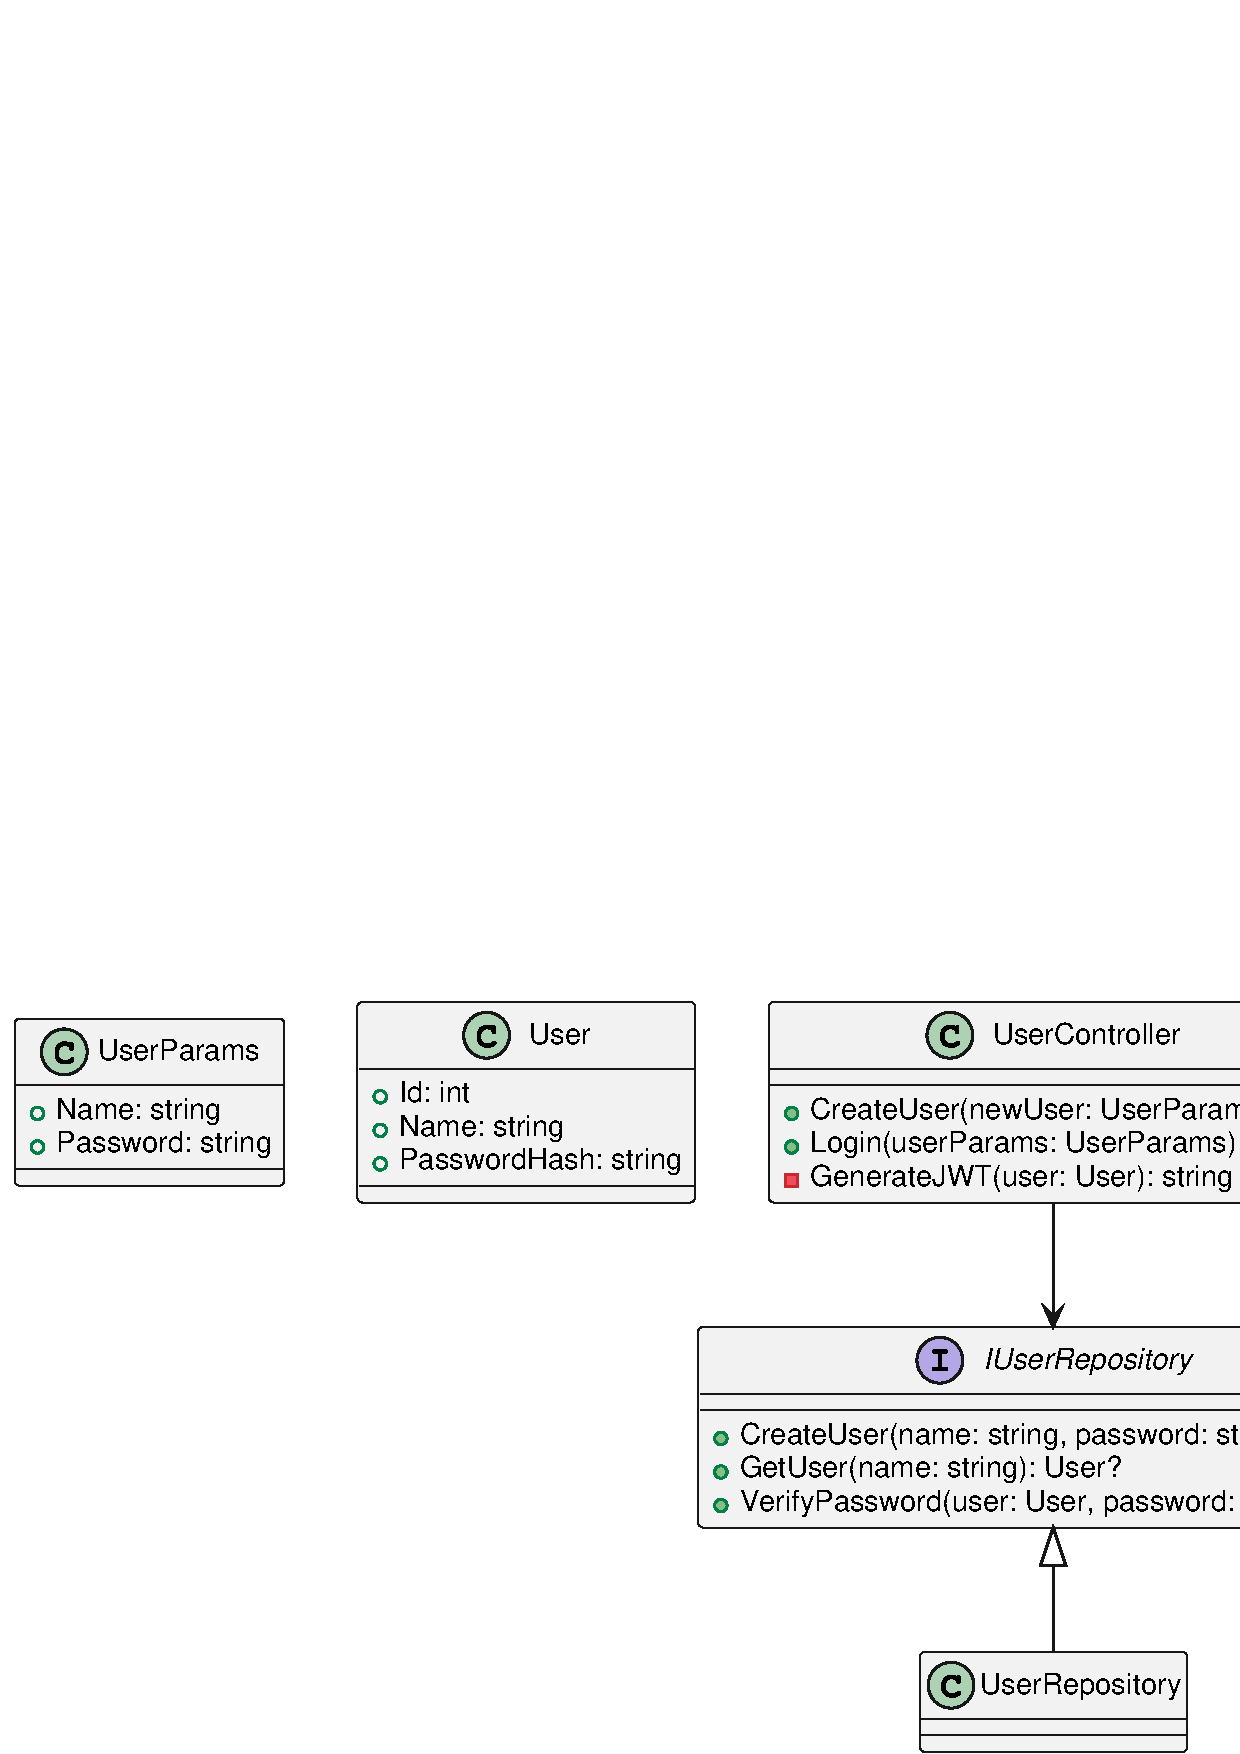
\includegraphics[width=\linewidth]{images/diagrams/auth.png}
    \end{center}
    \caption{}
    \label{fig:}
\end{figure}


\section{Aufsetzen (Deployment)}
